\section{Extended Introduction}
\label{sec:introduction}
Deep Learning (DL) models are becoming larger, and the increase in model size offers significant accuracy gain. In the area of Natural Language Processing (NLP), the transformers have paved way for large models like Bert-large (0.3B)~\cite{DBLP:journals/corr/bert}, GPT-2 (1.5B)~\cite{gpt-2}, Megatron-LM (8.3B)~\cite{megatronlm}, T5 (11B)~\cite{T5}. To enable the continuation of model size growth from 10s of billions to trillions of parameters, we experience the challenges of training them - they clearly do not fit within the memory of a single device, e.g., GPU or TPU, and simply adding more devices will not help scale the training.  

Basic data parallelism (DP) does not reduce memory per device, and runs out of memory for models with more than 1.4B parameters on current generation of GPUs with 32\,GB memory. Other existing solutions such as Pipeline Parallelism (PP), Model Parallelism (MP), CPU-Offloading, etc, make trade-offs between functionality, usability, as well as memory and compute/communication efficiency, but all of which are crucial to training with speed and scale. %(please see Sec.~\ref{sec:related-work} for more details). 

Among different existing solution for training large models, MP is perhaps the most promising. The largest models in the current literature, the 11B T5 model \cite{T5}, and Megatron-LM 8.3B \cite{megatronlm}, were both powered by model parallelism, implemented in Mesh-Tensorflow \cite{DBLP:journals/corr/mesh-tensor} and Megatron-LM\cite{megatronlm}, respectively. However, MP cannot scale much further beyond these models sizes. MP splits the model vertically, partitioning the computation and parameters in each layer across multiple devices, requiring significant communication between each layer. As a result, they work well within a single node where the inter-GPU communication bandwidth is high, but the efficiency degrades quickly beyond a single node \cite{megatronlm}. We tested a 40B parameter model using Megatron-LM across two DGX-2 nodes and observe about $5\,Tflops$ per V100 GPU (less than 5\% of hardware peak).    

So, how can we overcome the limitations of existing solutions and train large models more efficiently? To answer this question, we first analyze the full spectrum of memory consumption of the existing systems on model training and classify it into two parts:  1) For large models, the majority of the memory is occupied by \emph{model states} which include the optimizer states (such as momentum and variances in Adam~\cite{DBLP:journals/corr/Adam}), gradients, and  parameters. %(referred to as \emph{OGP} states in the paper). 
2) The remaining memory is consumed by activation, temporary buffers and unusable fragmented memory, which we refer to collectively as \emph{residual} states.
We develop \name --- Zero Redundancy Optimizer  --- to optimize memory efficiency on both while obtaining high compute and communication efficiency.
As these two parts face different challenges, we develop and discuss their solutions correspondingly.

{\bf Optimizing Model State Memory}
Model states often consume the largest amount of memory during training, but existing approaches such as DP and MP do not offer satisfying solution.  DP has good compute/communication efficiency but poor memory efficiency while MP can have poor compute/communication efficiency. More specifically, DP replicates the entire model states across all data parallel process resulting in redundant memory consumption;
while MP partition these states to obtain high memory efficiency, but often result in too fine-grained computation and expensive communication that is less scaling efficient.
Furthermore, all of these approaches maintain all the model states required over the entire
training process statically, even though not all model states are required all the time during
the training.
\begin{figure}[t!]
 \begin{center}
 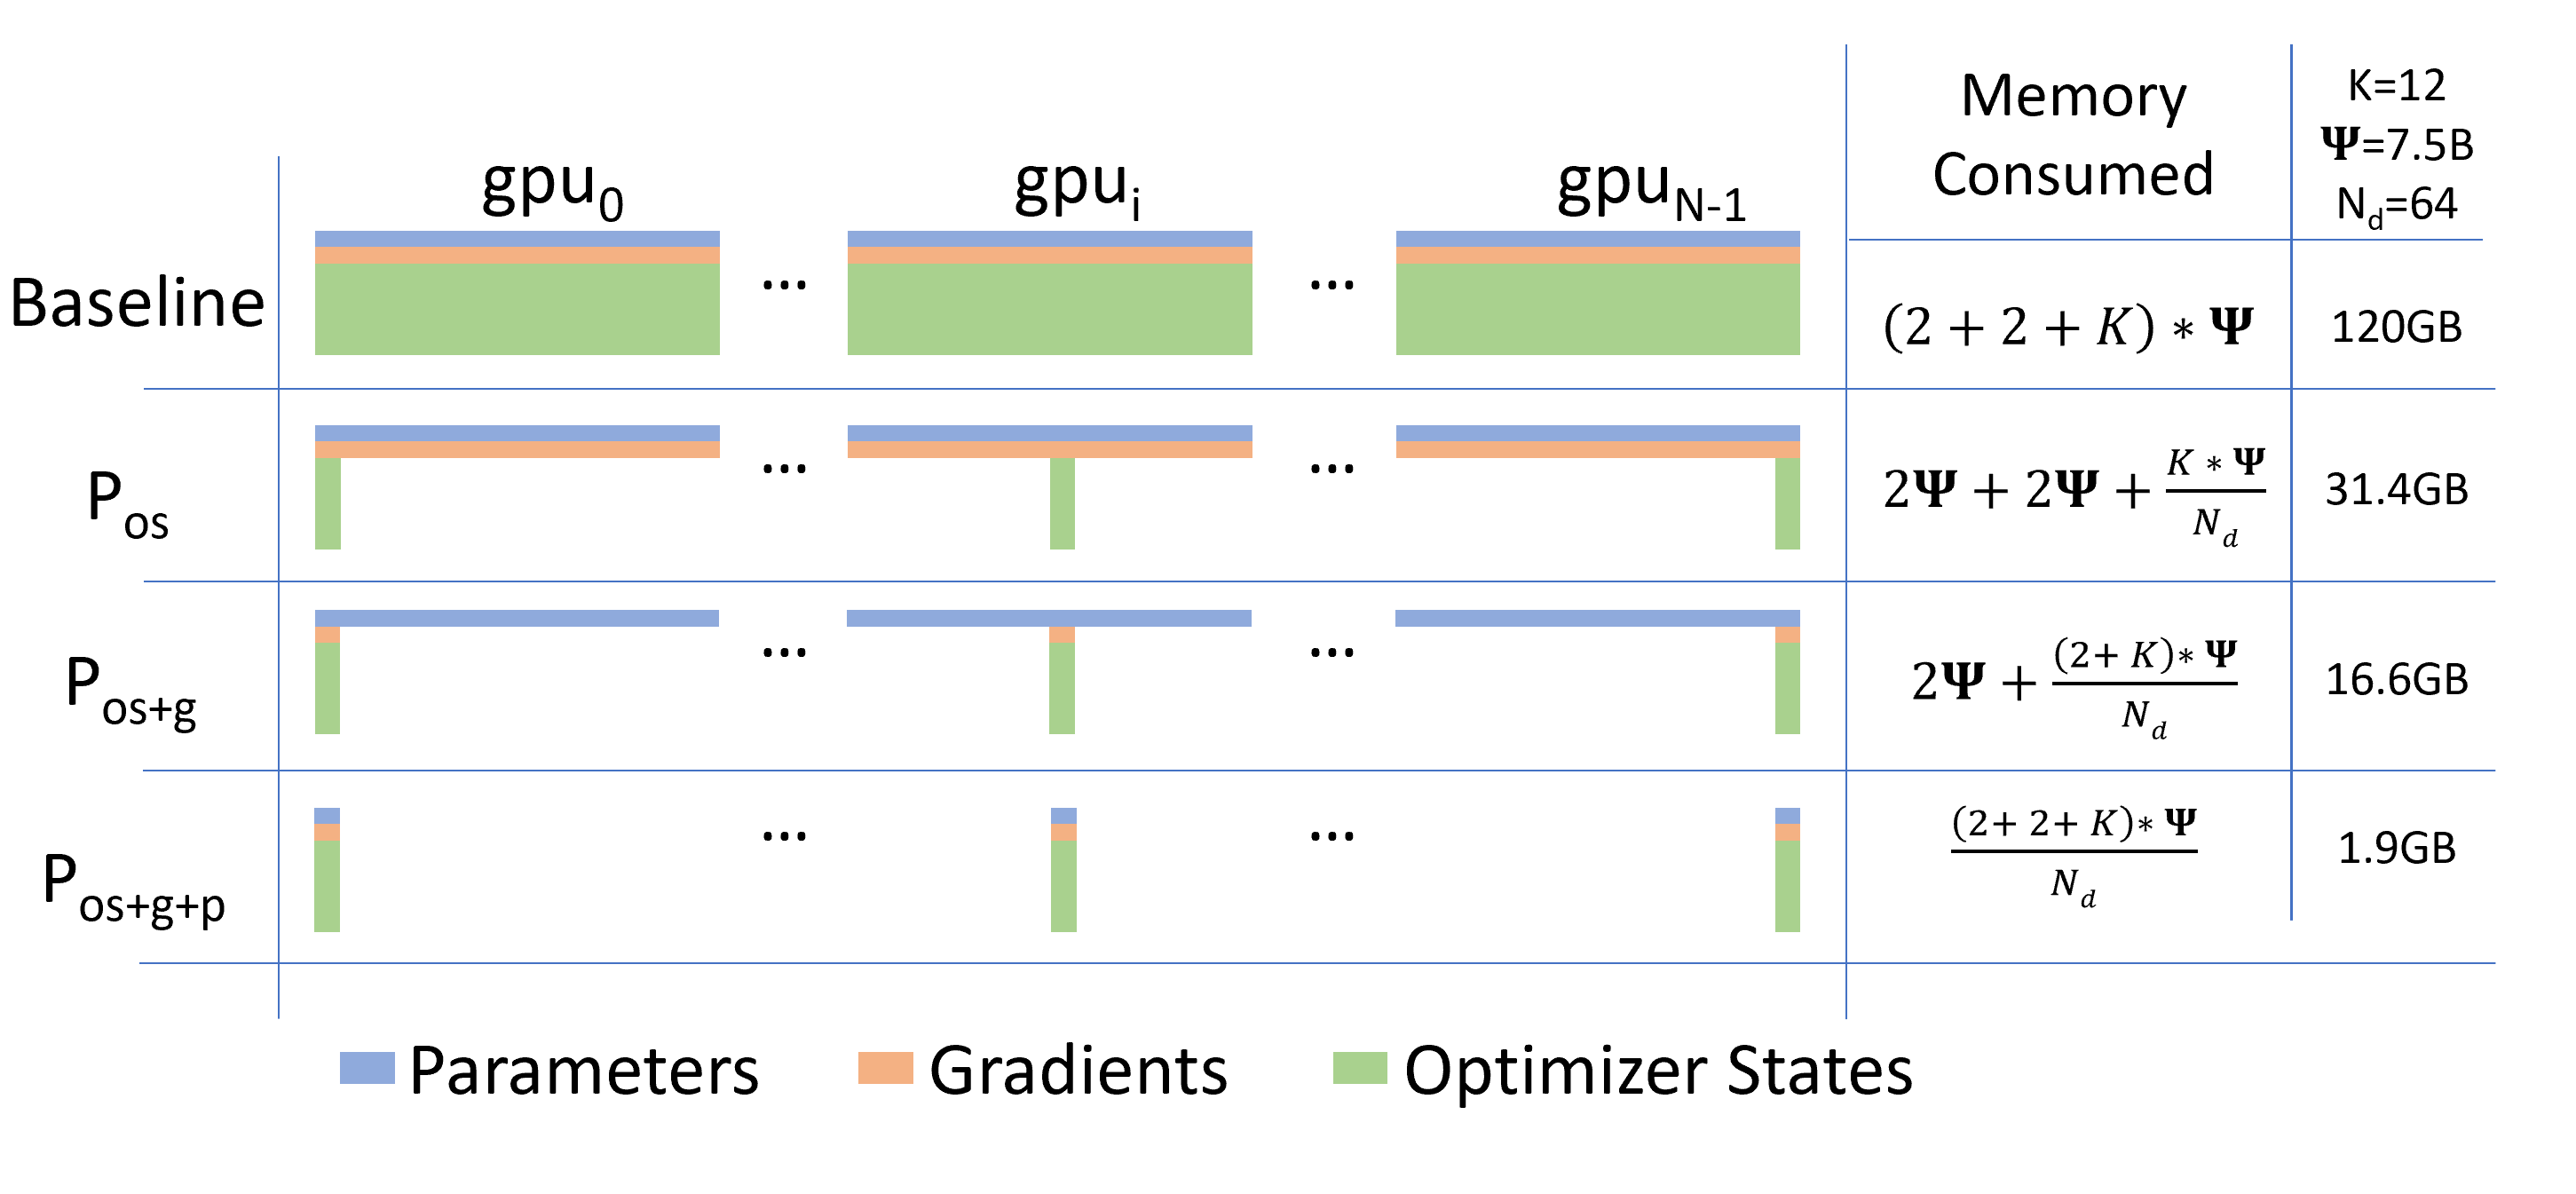
\includegraphics[width=1.0\columnwidth]{memory-consumption-v4.PNG}
 \caption{Comparing the per-device memory consumption of model states, with three stages of \name-DP optimizations. $\Psi$ denotes model size (number of parameters), $K$ denotes the memory multiplier of optimizer states, and $N_d$ denotes DP degree.  In the example, we assume a model size of $\Psi=7.5B$ and DP of $N_d=64$ with $K=12$ based on mixed-precision training with Adam optimizer. } 
 \label{fig:memory-consumption}
 \end{center}
 \end{figure}
Based on these observations, we develop \name-DP, ZeRO-powered data parallelism, that achieves the computation/communication efficiency of DP while achieving memory efficiency of MP.  \name-DP removes the memory state redundancies across data-parallel processes by \emph{partitioning} the model states instead of replicating them, and it retains the compute/communication efficiency by retaining the computational granularity and communication volume of DP using a dynamic communication schedule during training.  

\name-DP has three main optimization stages (as depicted in Figure \ref{fig:memory-consumption}), which correspond to the partitioning of optimizer states, gradients, and parameters. When enabled cumulatively:

1) Optimizer State Partitioning ($P_{os}$): 4x memory reduction, same communication volume as DP;

2) Add Gradient Partitioning ($P_{os+g}$): 8x memory reduction, same communication volume as DP; 

3) Add Parameter Partitioning ($P_{os+g+p}$): Memory reduction is linear with DP degree $N_d$. For example, splitting across 64 GPUs ($N_d$ = 64) will yield a 64x memory reduction. There is a modest 50\% increase in communication volume.

ZeRO-DP eliminates memory redundancies and makes the full aggregate memory capacity of a cluster available. With all three stages enabled, ZeRO can train a trillion-parameter model on just 1024 NVIDIA GPUs. A trillion-parameter model with an optimizer like Adam~\cite{DBLP:journals/corr/Adam} in 16-bit precision requires approximately 16 terabytes (TB) of memory to hold the optimizer states, gradients, and parameters. 16TB divided by 1024 is 16GB, which is well within a reasonable bound for a GPU (e.g., with 32GB of on-device memory).

%It reduces per-device memory footprint of a model \emph{linearly} with the increase in data parallelism degree while maintaining the communication volume close to that of the default data parallelism. \name-DP can fit models of \emph{arbitrary} size --- as long as there are sufficient number of devices to share the model states.  For example, our memory analysis shows that \name can fit a trillion parameter model on 1024 GPUs with data parallelism degree $N_d=1024$ (with more details in Section \ref{sec:summarymemoryoptimization}).

{\bf Optimizing Residual State Memory}
After \name-DP boosts memory efficiency for model states, the rest of the memory consumed by activations, temporary buffers, and unusable memory fragments could become a secondary memory bottleneck.  We develop \name-R to optimize the residual memory consumed by these three factors respectively.  

1) For activations (stored from forward pass in order to perform backward pass), we noticed checkpointing \cite{DBLP:journals/corr/ChenXZG16} helps but not sufficient for large models.  
Thus \name-R optimizes activation memory by identifying and removing activation replication in existing MP approaches through activation partitioning. It also offloads activations to CPU when appropriate.
%(see Sec.~\ref{sec:mp_activation_replication} for more details)

2) \name-R defines appropriate size for temporary buffers to strike for a balance of memory and computation efficiency. 

3) We observe fragmented memory during training due to variations in the lifetime of different tensors. Lack of contiguous memory due to fragmentation can cause memory allocation failure, even when enough free memory is available. \name-R proactively manages memory based on the different lifetime of tensors, preventing memory fragmentation.

%\name-R not only reduces memory usage but also improves training efficiency as we show in Sec.\ref{sec:evaluation}. 
\name-DP and \name-R combined together forms a powerful system of memory optimizations for DL training that we collectively refer to as \name.

\textbf{\name and MP}: Since \name eliminates the memory inefficiency in DP, it is natural to ask: Do we still need MP, and when?  How does \name work with MP?  With \name, MP becomes a less attractive option for the purpose of fitting large models alone.  \name-DP is at least as effective on reducing per-device memory footprint as MP, or more effective sometimes when MP cannot divide the model evenly. It also has comparable or better scaling efficiency. Furthermore, data parallelism is so easy to use that it is widely applicable across different workloads, while MP approaches today often need some work from model developers to revise their model, system developers to work out distributed operators, and existing work like Megatron-LM only supports a limited set of operators and models.

That being said, there are still cases where we want to leverage MP: i) When used with \name-R, MP can reduce activation memory footprint for very large models. ii) For smaller models where activation memory is not an issue, MP can also have benefits when aggregated batch size using DP alone is too big to have good convergence.\footnote{Prior work \cite{DBLP:journals/corr/batch-scaling} shows, very large batch size could slow down convergence.  For given model and data, there is a measure of critical-batch size, where increasing batch size further slows down convergence.  The detailed discussion of this topic is beyond the scope of the paper.}  In those case, one can combine \name with MP to fit the model with an acceptable aggregated batch size.

We show that \name can be combined with MP, resulting in a max theoretical memory reduction of $N_d \times N_m$ times on each device with a DP degree of $N_d$ and MP degree of $N_m$. 
This could allow us to fit a trillion parameter model on 1024 GPUs with 16-way model parallelism (within each DGX2 node) and 64-way data parallelism across nodes, and run it efficiently using a modest batch size!


\begin{figure}[t!]
 \begin{center}
 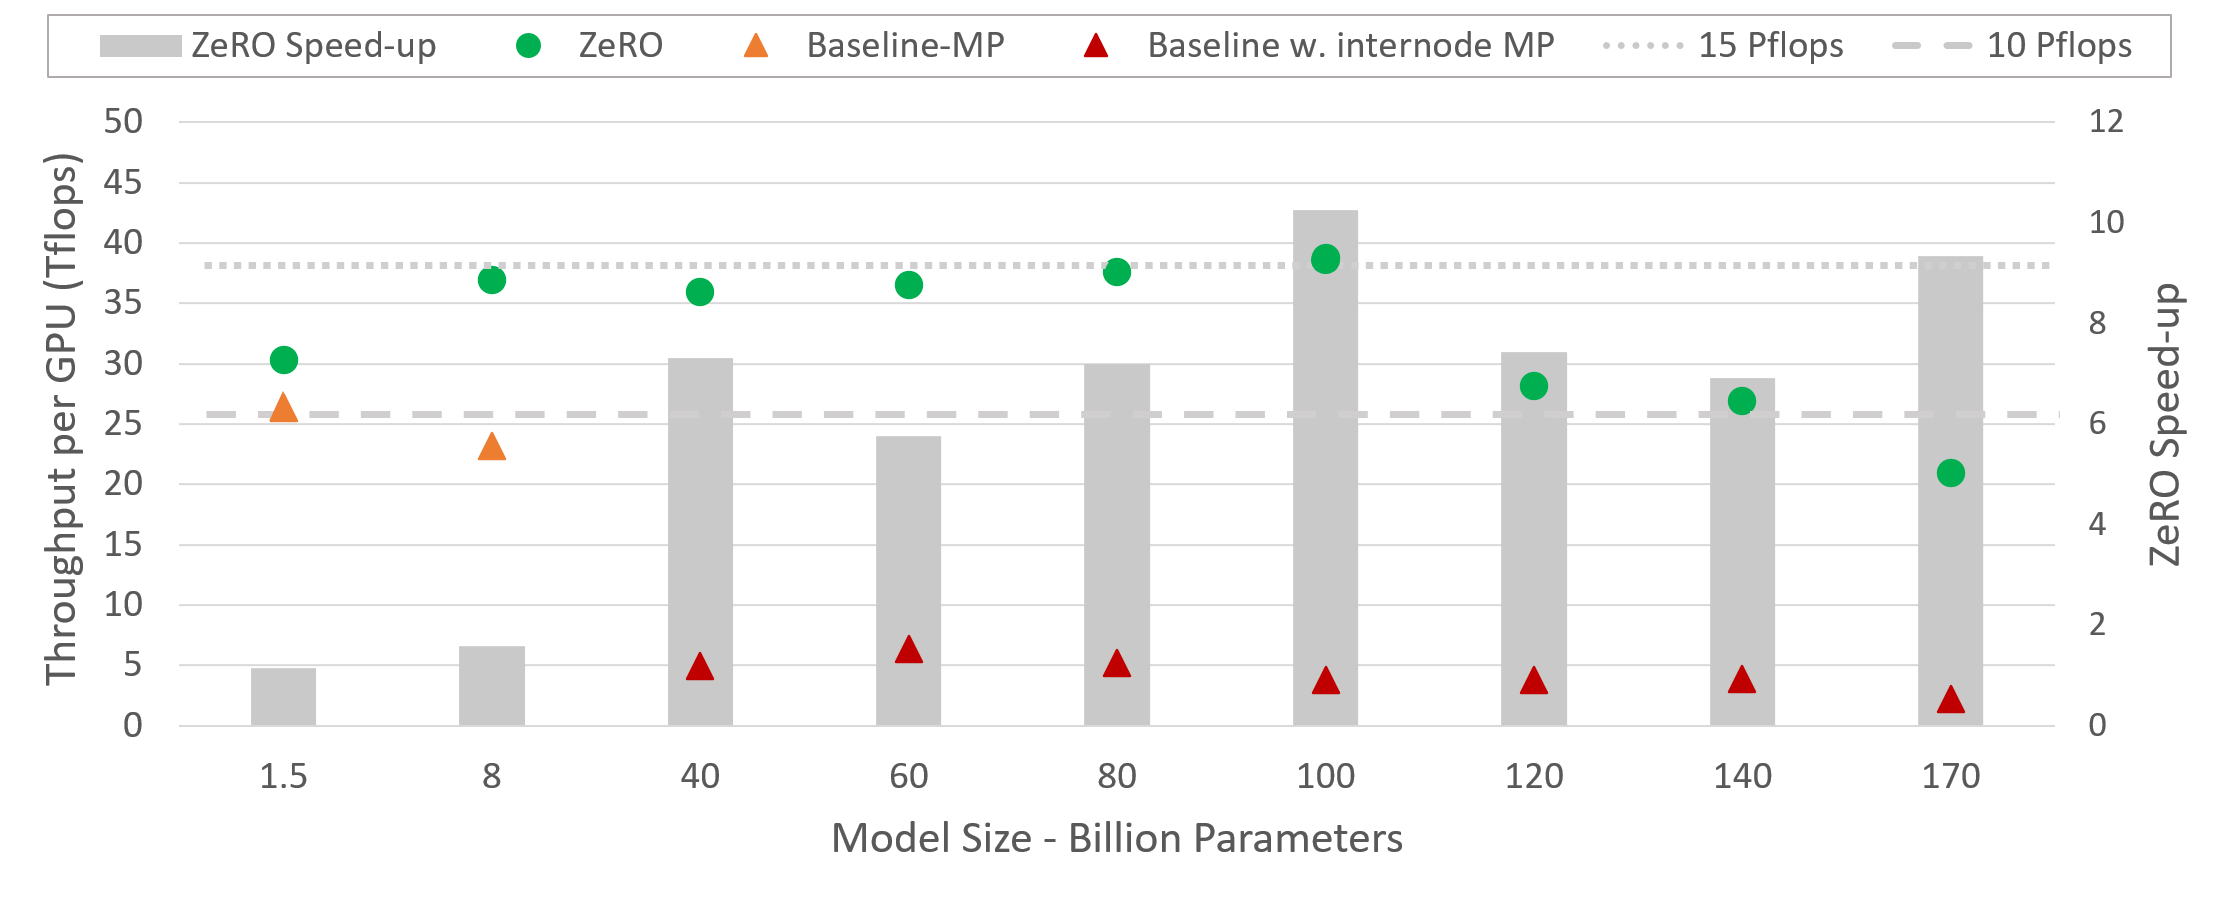
\includegraphics[width=1.0\columnwidth]{model_size_and_speedup.PNG}
 \caption{\name training throughput and speedup w.r.t SOTA baseline for varying model sizes.  For \name, the MP always fit in a node, while for baseline, models larger than 40B require MP across nodes.} 
 \label{fig:billion_parameter_speedup}
 \end{center}
 \end{figure}

\begin{figure}[t!]
 \begin{center}
 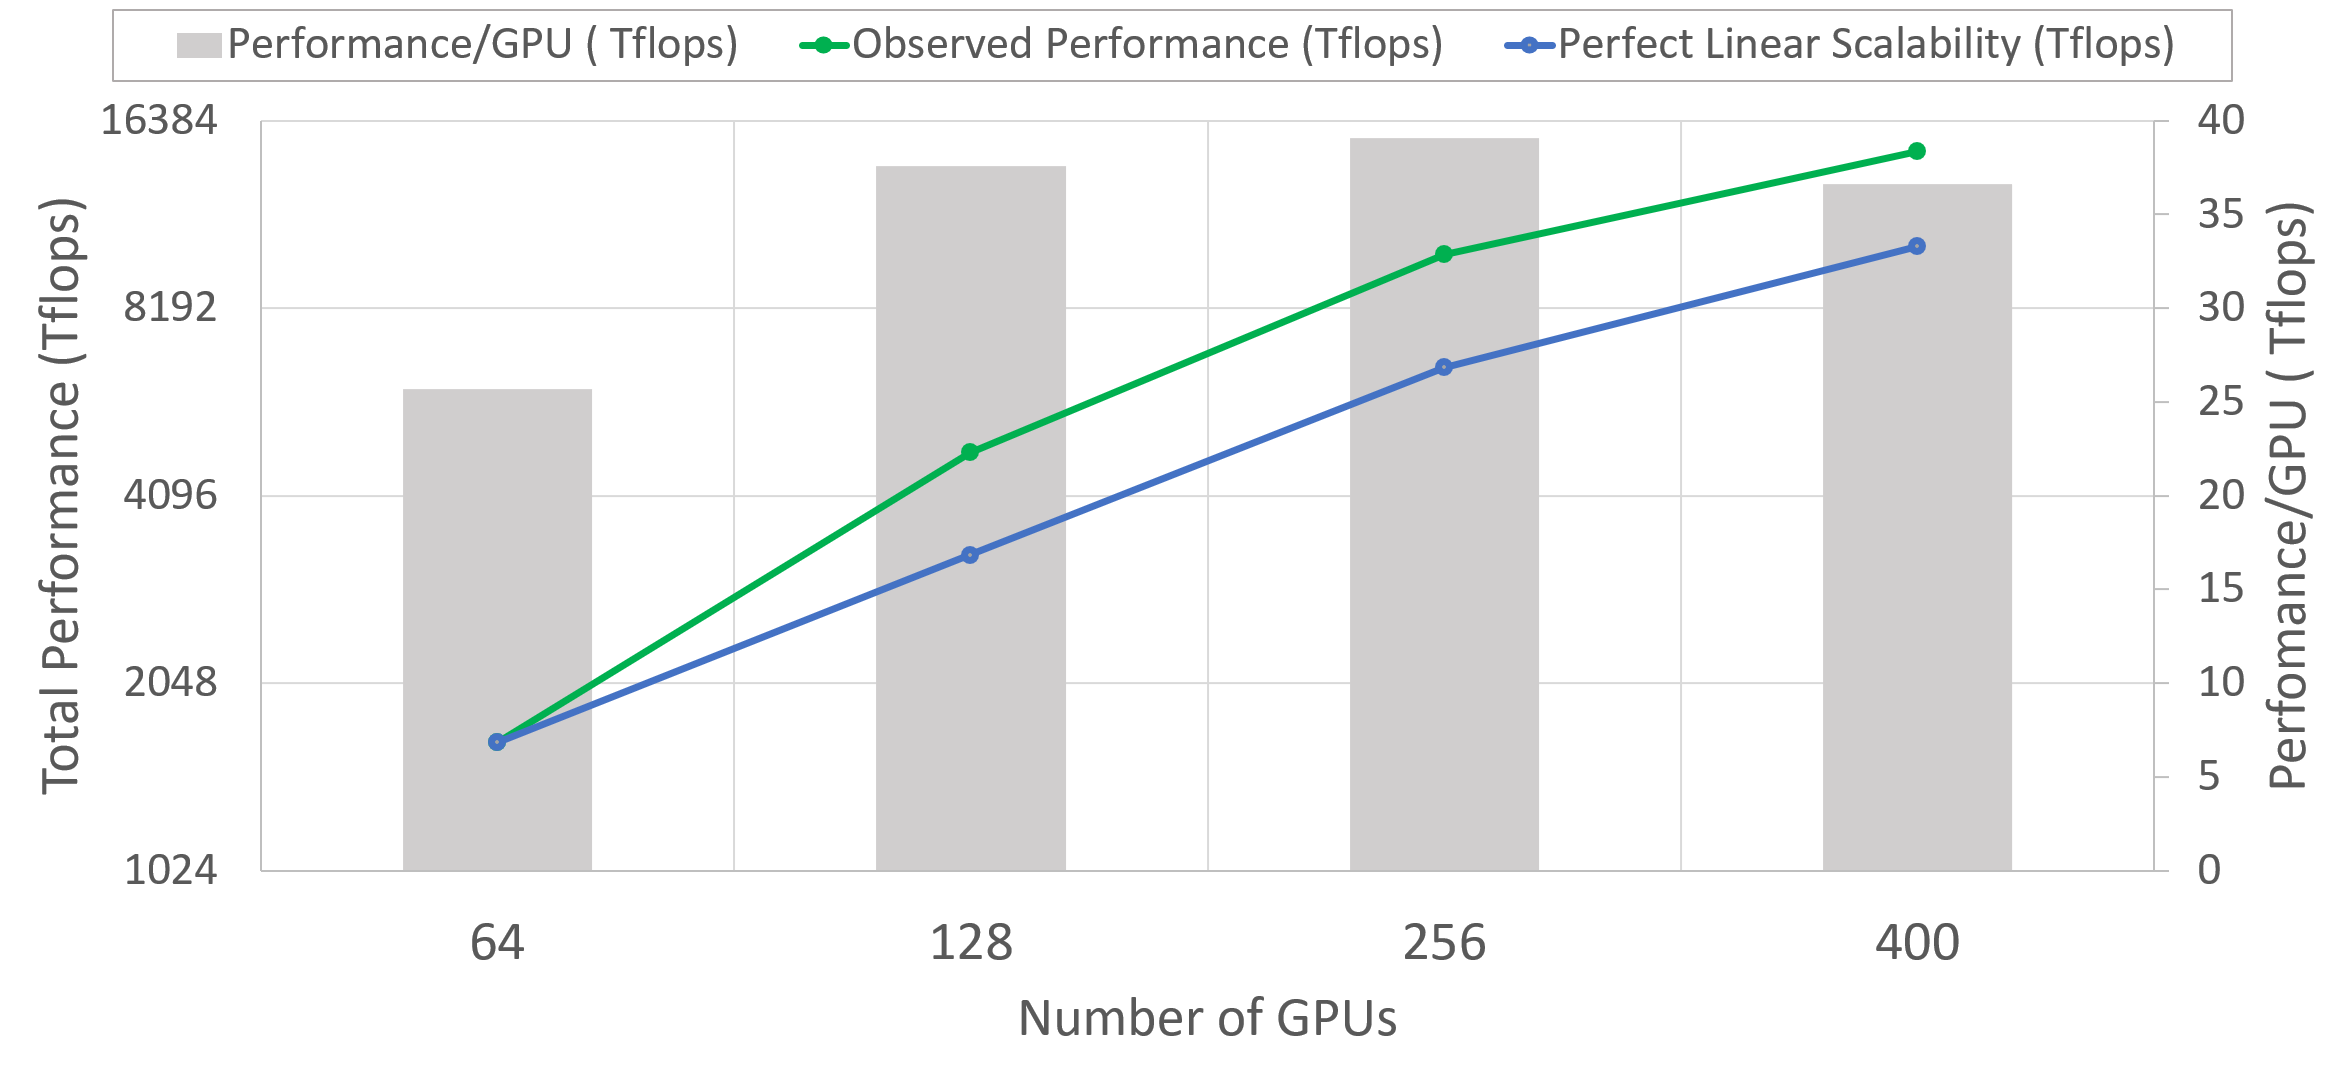
\includegraphics[width=1.0\columnwidth]{hyperscale_60B_model_v2.PNG}
 \caption{Superlinear scalability and per GPU training throughput of a 60B parameter model using \name-100B.} 
 \label{fig:hyperscale_60B}
 \end{center}
 \end{figure}

% \begin{figure*}[t!]
%     \centering
%     \begin{minipage}{.55\textwidth}
%         \centering
%         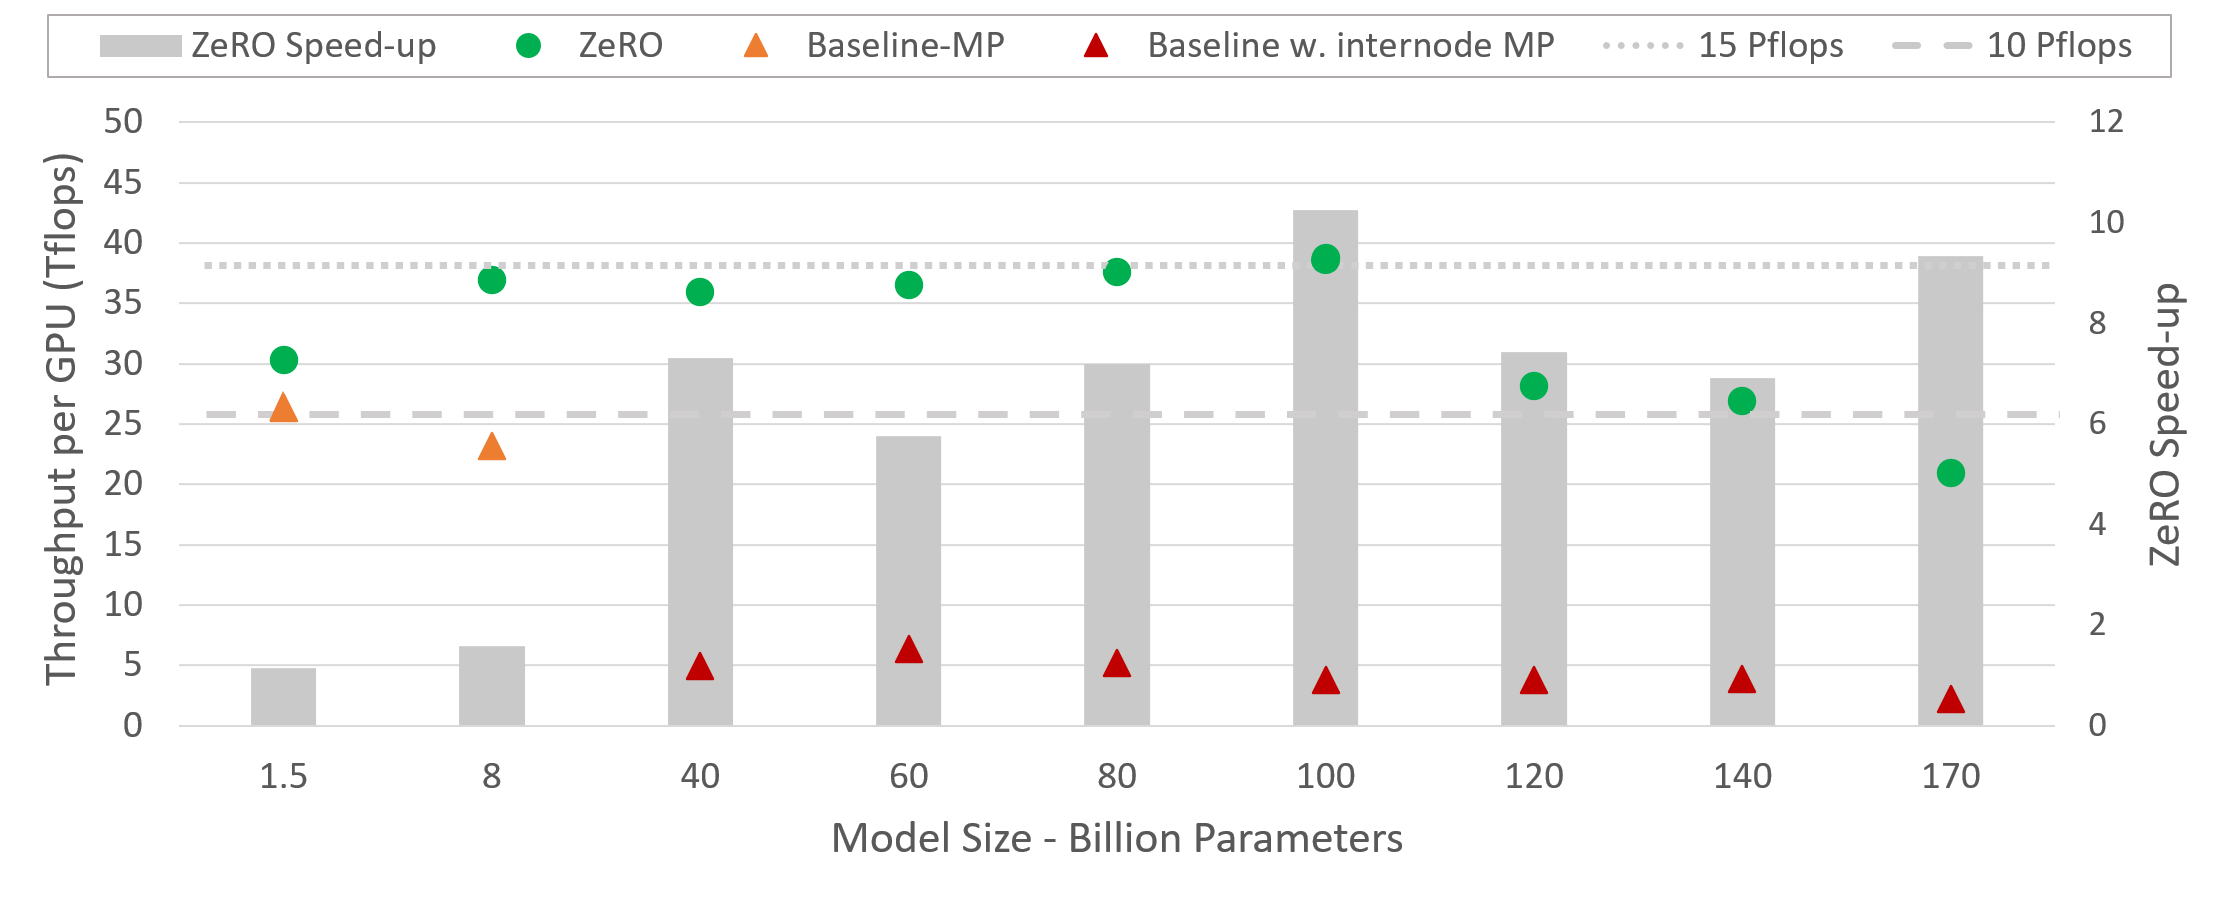
\includegraphics[width=\linewidth]{model_size_and_speedup.PNG}
%         \caption{\name training throughput and speedup w.r.t SOTA baseline for varying model sizes.  For \name, the MP always fit in a node, while for baseline, models larger than 20B require MP across nodes. }\label{fig:billion_parameter_speedup}
%     \end{minipage}
%     \quad
%     \begin{minipage}{.4\textwidth}
%         \centering
%         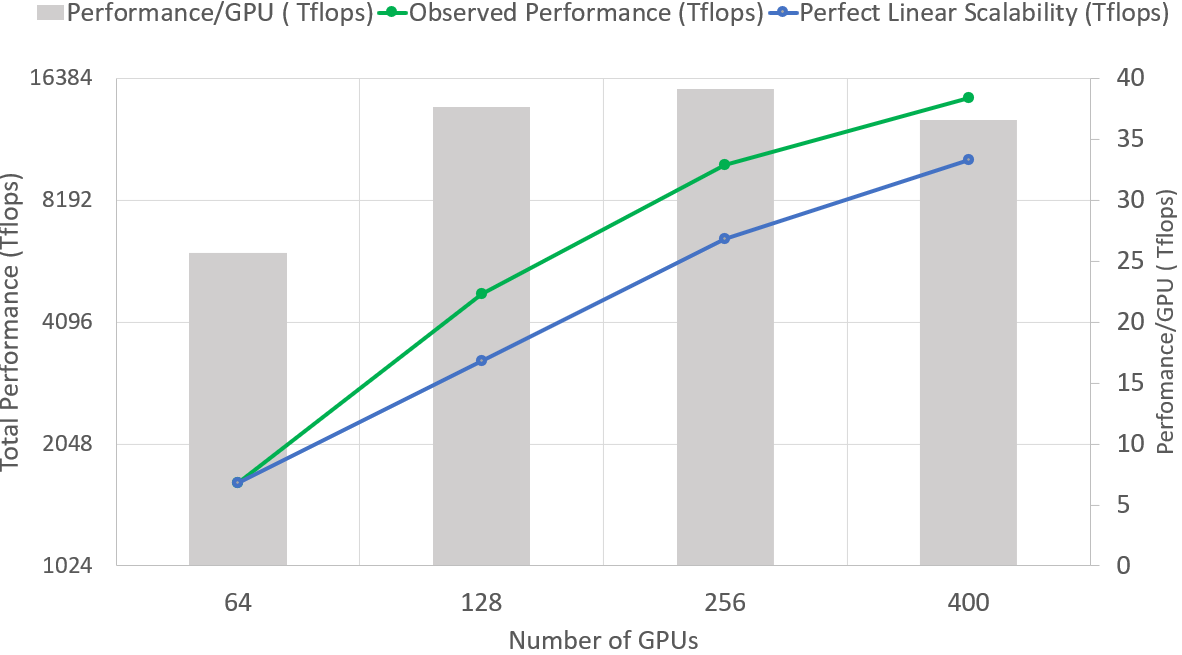
\includegraphics[width=\linewidth]{hyperscale_60B_model.PNG}
%         \caption{Superlinear scalability and per GPU training throughput of a 60B parameter model using \name-100B.}\label{fig:hyperscale_60B}
%     \end{minipage}
% \end{figure*}

{\bf Implementation \& Evaluation}
The complete set of optimizations in \name could allow us to run models with trillion parameters on the high-end hardware cluster today (e.g., with 1K V100 GPUs), however, the hardware compute capacity is still too limited and training time can be impractically long ($>$1 year).  Therefore, our focus for this implementation is to efficiently support models with 10x parameters ($\sim$100B parameters) than state-of-the-art (SOTA) while still being within reach of the compute capabilities of current hardware. We implement and evaluate a subset of optimizations in \name called \name-100B --- $P_{os+g}$ of \name-DP plus ZeRO-R --- that allow us to achieve this goal. The results show:

\underline{Model Size} Combined with MP, \name-100B runs 170B parameter models efficiently, while the existing system like using Megatron alone cannot scale efficiently beyond 40B parameters, as shown in Figure~\ref{fig:billion_parameter_speedup}.
This is an over 8x increase in model size compared to SOTA.

\underline{Speed} Improved memory efficiency powers higher throughput and faster training. 
As shown in Figure~\ref{fig:billion_parameter_speedup}, \name runs 100B parameter models on a 400 Nvidia V100 GPU cluster with over 38 TFlops per GPU, and aggregate performance over 15 Petaflops. This is more than 10x improvement in training speed compared to SOTA for the same model size.

\underline{Scalability} We observe super linear speedup in the regime of 64-400 GPUs, where the performance more than doubles when we double the number of GPUs. This is a property of \name-DP which reduces the memory footprint of the model states as we increase the DP degree allowing us to fit larger batch sizes per GPU resulting in better performance. We expect this behaviour to continue further as we increase the number of GPUs beyond 400.

\underline{Democratization of Large Model Training} \name-100B powers data scientist to train models with up to 13B parameters without any MP or PP that requires model refactoring, where 13B is more parameters than the largest model in literature (T5 with 11B parameters). Data scientists can thus experiment freely with large models without worrying about parallelism. In comparison, exist systems (e.g., PyTorch Distributed Data Parallel) runs out of memory with 1.4B parameter models. 
%Furthermore, MP requires high-bandwidth interconnect such as NVLINK/NVSwitch; \name-100B allows them to be trained more efficiently on clusters that don't have these high-end intra-node interconnect.

\underline{New SOTA Model} \name powers the largest language model with 17B parameters and record-breaking accuracy, Turing-NLG~\cite{t-nlg}.
%records in the world --- with significantly more parameters that the T5 11B \cite{T5} model --- establishing the new SOTA not just in model size but also in terms of accuracy in its category (details hidden to adhere to double-blind policy). 



\begin{comment}
\textbf{Contributions}
Our contributions are as follows:
\begin{itemize}
    \item \name, a powerful system of memory optimizations that reduces the memory footprint of the model states proportional to the data parallelism degree and those of the activations proportional to the model parallelism degree. Additionally, it also performs on the fly memory de-fragmentation to increase the usable memory and improve training efficiency
    \item Enables training models with over 13B parameter model without any model parallelism. As an implication, the largest model before this work, T5 \cite{T5} with 11B parameters can be trained without any model parallelism using \name.
    \item Enables training models with over 170B parameters using a combination of ZeRO and model parallelism. For comparison, the largest model that can be trained using Megatron, the state-of-art model parallelism framework on current generation of hardware is about 20B. This is over 8x increase in model size.
    \item Extensive evaluation of the performance of \name in comparison to SOTA for models ranging from 1.5B to 170B on a 400GPU V100 Cluster. \name achieves up to 10x speedup, while achieving over 15 Petaflops in sustained performance. 
    \item \name makes super-linear scaling possible for large models by enabling the increase of batch size per GPU with increase in data parallelism degree. This is possible with \name because the memory consumption of model states decreases with the increase in data parallelism.
    \item \name democratizes large scale training by enabling high performance for large models on modest clusters without requiring high end interconnect fabric such as NVLINK or NVSWitch required by model parallel frameworks such as Megatron to achieve good performance.
    \item \name enables the training of the worlds largest and the most powerful language model (LM), the 17.2B parameter Turing-NLG model establishing the new SOTA for LM.
\end{itemize}
\end{comment}
We share \name as a part of our open source DL training optimization library called DeepSpeed\footnote{https://github.com/microsoft/deepspeed}.
We plan to release all implementations described in this paper by end of May 2020 and extend it further to support 1 trillion parameters by enabling \name-DP stage 3 partitioning parameters ($P_{os+g+p}$). We plan to make \name fully accessible to the DL community to catalyze the evolution and democratization of large model training at scale.  
 
%The rest of the paper is organized as follows: ....
% Running a model with a trillion parameters efficiently is no longer impossible,  but quite feasible!

%[a connection would help]
%AlthoTraining a trillion parameter model is feasible with \name but on today's cluster of about a thousand GPUs (and 100 petaflops of compute power), it will take at least several months.   with the current compute power, requiring exaflops of hardware clusters to 
\begin{comment}





With this goal, we implemented the first two stages of ZeRO, optimizer state partitioning and gradient partitioning for model states as well as the optimizations on activation, temp buffers and memory defragmentation, which we call ZeRO-OGR.  



\name has three main optimization stages: partitioning (1) optimizer states, (2) gradients and (3) parameters which bring memory savings of 4, 8 and $N_d$ times respectively for a popular training optimizer like ADAM, when compared using data parallelism only or combination of data and model parallelism. For instance, state-of-the-art data + model parallelism implementation, Megatron, supports about 20B parameter model training on a cluster of DGX-2 nodes, while these three stages of optimization will enable training ~80B, ~160B, and arbitrary model sizes ($N_d \times 20$B), respectively.      

As the first step of the evaluation, we implemented optimizer state partitioning (Stage 1, $P_{os}$) on top of PyTorch and call this version \nameos.  We demonstrate its capability to support 80-100B parameter models, which we hope will address the near-term growth on model size.  
The experimental results with \nameos show that: 
\begin{itemize}
    \item Without any model-parallelism, \nameos-\emph{powered} data-parallelism enables training models with up to 6B parameters on V100 GPUs (32GB of device memory) while existing systems (e.g., PyTorch Distributed Data Parallel) runs out of memory with 1.5B parameter models. \nameos gives 4x memory saving / model size boost. Model developers can run up to 6B parameter models without worrying about model parallelism.
    %\item Combined  with  model  parallelism, \name-$P_{os}$ runs 80B parameter  models efficiently,  while  the  existing  system  like  Megatron  exhibits poor scaling for 20B+ parameter models.
    \item Combined  with  model  parallelism, \nameos runs 80B parameter models efficiently, while the existing system like using Megatron alone cannot scale efficiently beyond 20B parameters, as shown in Figure \ref{fig:billion_parameter_model_feasibility}. \nameos also fits 100B parameter models without requiring inter-node model parallelism.
    \item Improved memory efficiency from \nameos also helps run models more efficiently (e.g., by allowing smaller model parallelism degree and higher batch size): we demonstrate up to 6x throughput gain for GPT-like models with various sizes spanning 1.5B to 100B.
    %GPT2 (1.5B) and its variations with 8B and 20B parameters. 
\end{itemize}
 
%Figure \ref{fig:billion_parameter_model_feasibility} visualizes the improvement of \nameos: comparing with state of arts, we 
We will share the code repository for \nameos soon. Over time, we will release the full implementation with the remaining two stages of \name to support training models with trillions of parameters.  With \name, we aim to transform large models from infeasible-to-train to feasible- and efficient-to-train.    
%Moving forward, we hope to power all optimizations of \name and continue to push the boundary of training system capability      

\begin{figure}[t!]
 \begin{center}
 %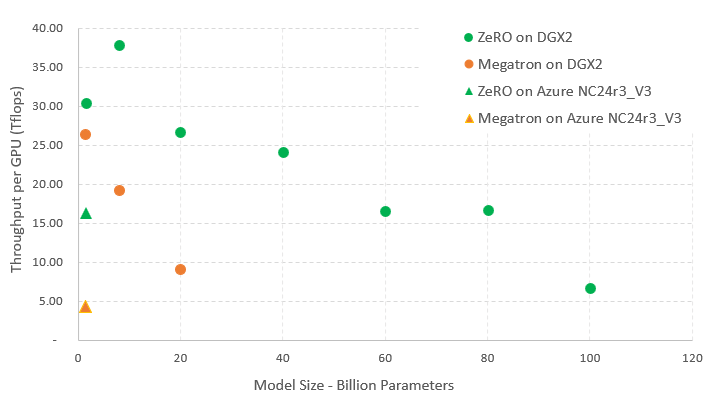
\includegraphics[width=1.0\columnwidth]{billion_parameter_model_feasibility.PNG}
 %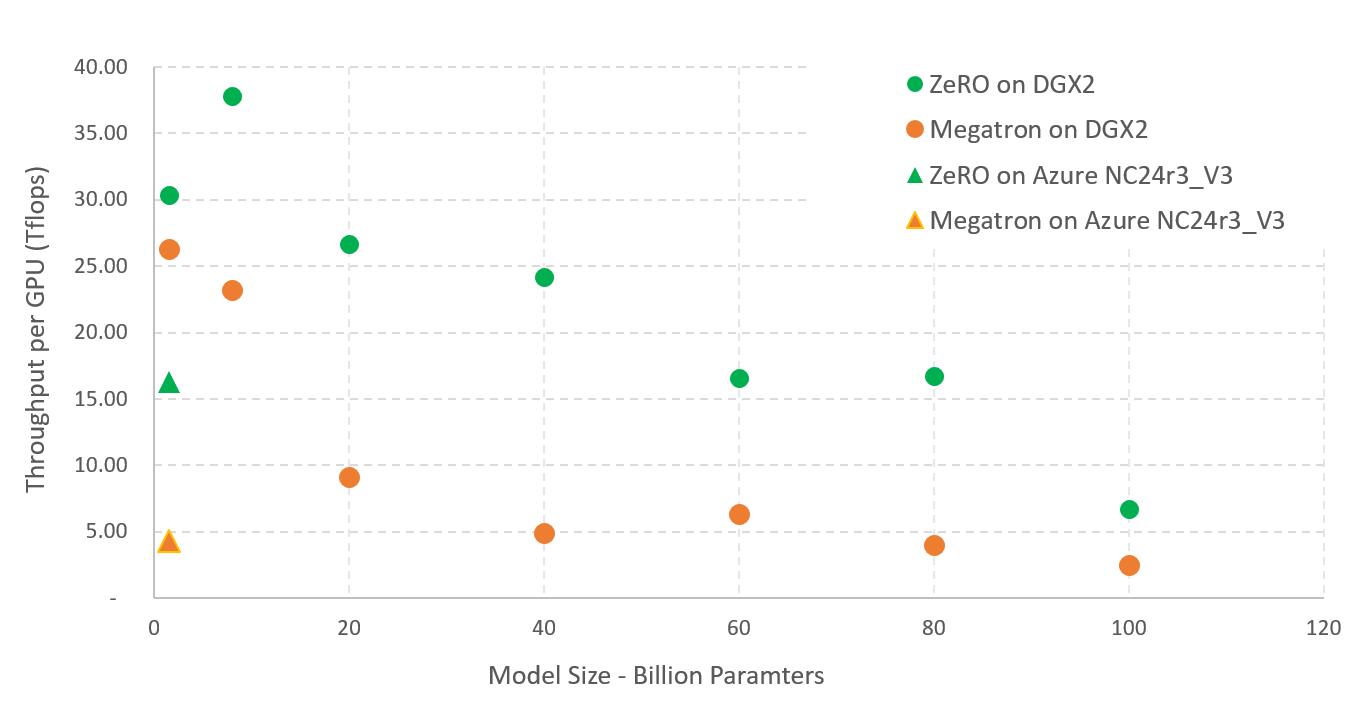
\includegraphics[width=1.0\columnwidth]{zero_w_internode_megatron.PNG}
 %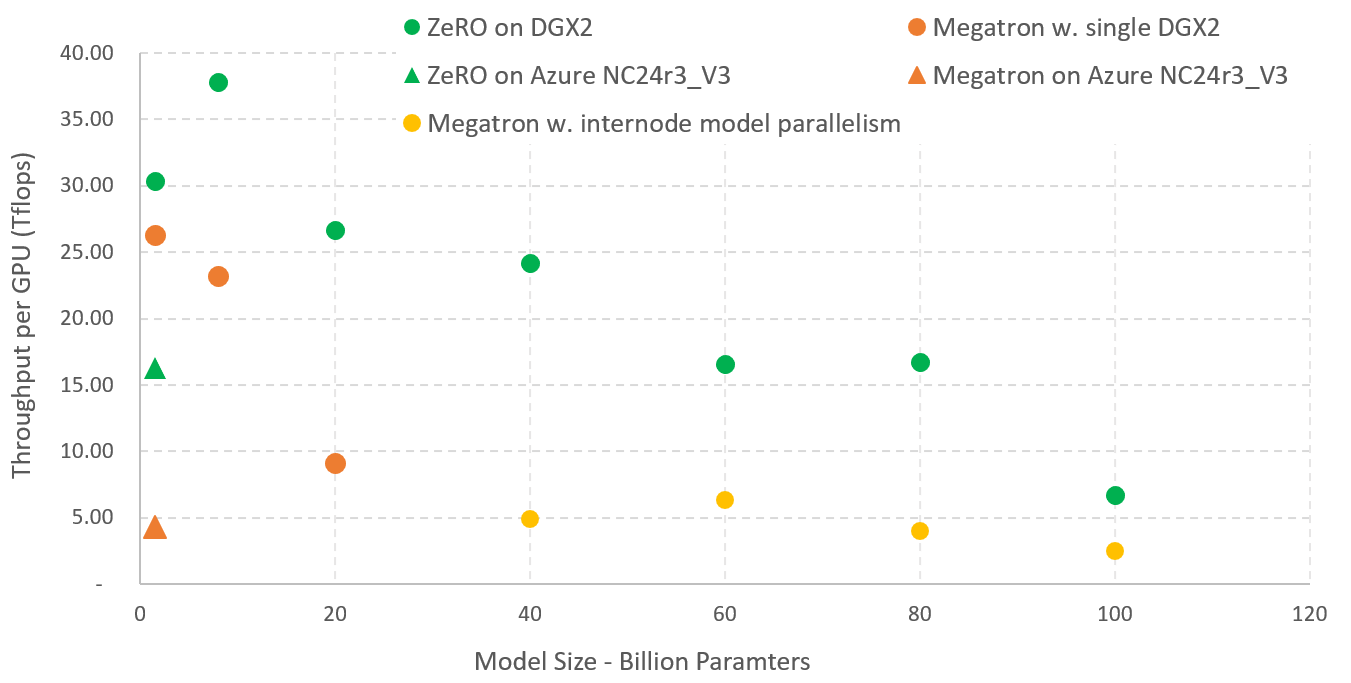
\includegraphics[width=1.0\columnwidth]{zero_w_internode_megatron_v2.PNG}
 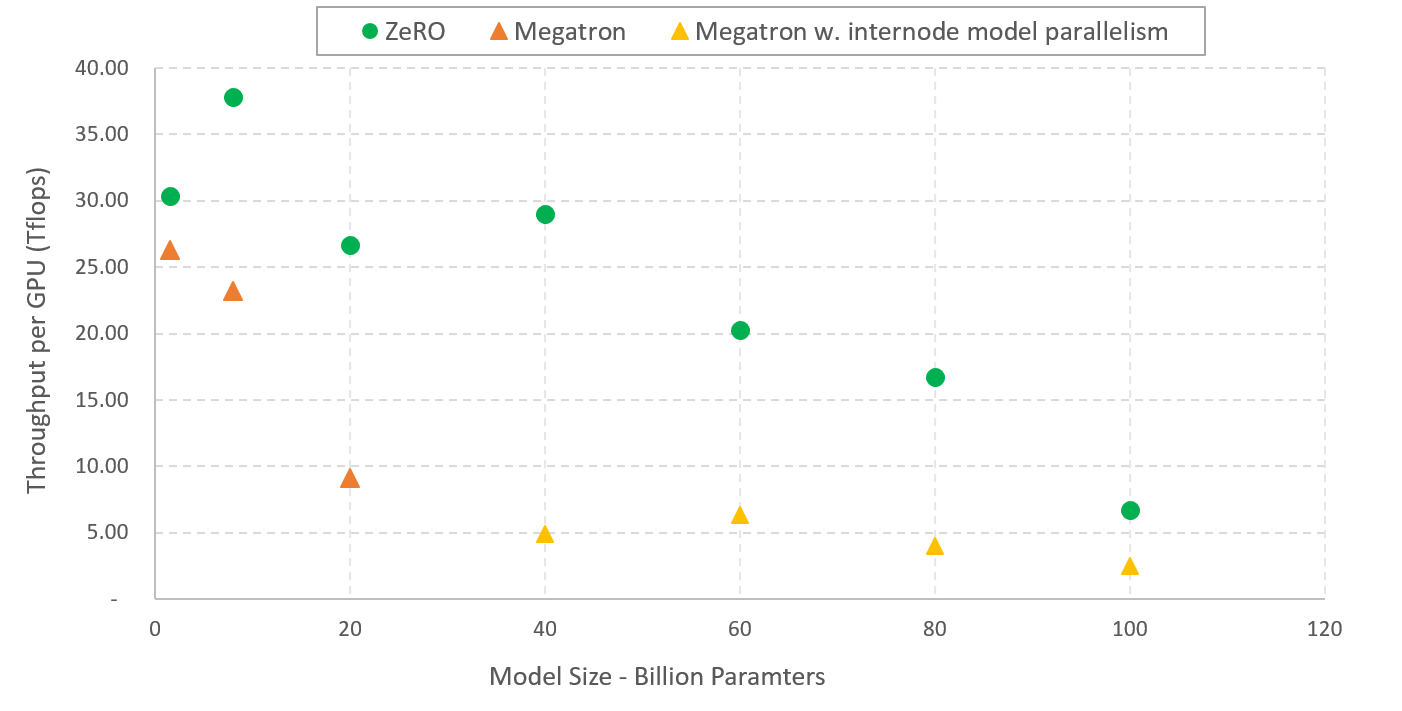
\includegraphics[width=1.0\columnwidth]{zero_w_internode_megatron_v2_woAzure.PNG}
 \caption{Comparing \nameos with Megatron on the runnable model sizes and throughput. All experiments are conducted using the smallest model parallelism degrees possible. For \nameos, the model parallelism degree always fit within a single node, while for Megatron, models larger than 20B require model parallelism across nodes.  Further details on experimental setup and configurations are in Section \ref{sec:evaluation}.  %enables efficient training of up to 80 billion parameter models that were previously inefficient to train with existing systems such as Megatron which does not scale beyond 20 billion parameter models. {\color{green} [as the first figure, this caption needs to be self contained.]}  
 } 
 \label{fig:billion_parameter_model_feasibility}
 \end{center}
 \end{figure}
\end{comment}

%We take a step back to first example the memory consumption of the current training system.
%We observe that the memory consumption of the state-of-art approach is far from optimal.  For example,  a 1.5B parameter GPT-2 model has its weights (or parameters) taking 3GB of memory in 16-bit training, yet, it cannot be trained on a single GPU with 32GB memory using Tensorflow or Pytorch.  As another example, Megatron can train up to a 20B parameter model on 16 V100 GPUs \cite{large model on V100}. However, the size of the model weights (40GB in 16-bit) is far smaller than the total available aggregated memory of the 16 GPUs (32GB-per-GPU x 16 = 512 GB).

%the current state-of-art is far from optimal. The state-of-art tensor slicing implementation for NVIDIA called  Megatron can train up to an 20B parameter model on 16 NVIDIA V100 GPUs \cite{large model on V100}. However, it is interesting to observe that, the size of the model (40GB in 16-bit) is far smaller than the total available memory on 16 V100 GPUs (32GB-per-GPU x 16 = 512 GB). As another example, a 1.5B parameter GPT-2 model has a memory footprint of only 3GB in 16-bit, yet, it cannot be trained on a single GPU with 32GB memory using Tensorflow, or Pytorch. Megatron requires a minimum of 2 V100 GPUs to execute it without running out of memory. [This part is a bit tricky, as we cannot run it using less than 2 GPUs either since we need to use data parallelism.]

%Given this gap between the memory footprint of the trainable models and the available GPU memory, it is only natural to ask, where is all the memory going? 

\begin{comment}


Given the significant gap between how `little' memory the parameters alone of the largest trainable model consumes vs how `much' aggregated memory the devices hold, it is only natural to ask, where all the memory goes? 

In this paper, we break down and analyze the memory consumption of training large deep learning models using existing approaches.  Beyond storing parameters, other states such as gradients and 


We identify the prominent source of memory inefficiency at data parallelism --- all of the data-parallel device instances replicate the parameters, gradients, and other optimizer states such as momentum and variance --- which incurs so much redundancy / waste on the memory consumption.    
Instead of replicating them, partitioning them would reduce memory consumption significantly. 

We propose a set of techniques   

, and using this understanding, we develop a set of inter-connected techniques that we collectively call \name (Zero Redundancy Optimizer) which allows us to train significantly larger models on the same amount of aggregate memory than currently possible. More concretely, we demonstrate that on a 400 V100 GPU cluster with 25 DGX-2 boxes, we can train an extremely large 100B parameter model with no computational performance degradation, compared to Megatron which will run out of memory over 20B parameters or incur significant performance degradation. Furthermore, we can train an unprecedented 1 Trillion parameter model at the cost of doubling the communication volume, and minimal performance impact. 

The \name technology paves the way to train new generation of large models on current generation hardware, and holds the promise for exa-scale training on new generation of super-computers. In this paper we describe \name and compare it to Megatron in terms of memory consumption as well as performance.

The paper is organized as follows: First we give a background on how large models are currently trained using a combination of data parallelism and model parallelism. Next, we provide insights on the total memory consumption during DL training. Based on the insights, we the develop /name to reduce the memory consumption during training. 
\end{comment}
